\documentclass{book}
\usepackage[a4paper,top=2.5cm,bottom=2.5cm,left=2.5cm,right=2.5cm]{geometry}
\usepackage{makeidx}
\usepackage{natbib}
\usepackage{graphicx}
\usepackage{multicol}
\usepackage{float}
\usepackage{listings}
\usepackage{color}
\usepackage{ifthen}
\usepackage[table]{xcolor}
\usepackage{textcomp}
\usepackage{alltt}
\usepackage{ifpdf}
\ifpdf
\usepackage[pdftex,
            pagebackref=true,
            colorlinks=true,
            linkcolor=blue,
            unicode
           ]{hyperref}
\else
\usepackage[ps2pdf,
            pagebackref=true,
            colorlinks=true,
            linkcolor=blue,
            unicode
           ]{hyperref}
\usepackage{pspicture}
\fi
\usepackage[utf8]{inputenc}
\usepackage{mathptmx}
\usepackage[scaled=.90]{helvet}
\usepackage{courier}
\usepackage{sectsty}
\usepackage{amssymb}
\usepackage[titles]{tocloft}
\usepackage{doxygen}
\lstset{language=C++,inputencoding=utf8,basicstyle=\footnotesize,breaklines=true,breakatwhitespace=true,tabsize=4,numbers=left }
\makeindex
\setcounter{tocdepth}{3}
\renewcommand{\footrulewidth}{0.4pt}
\renewcommand{\familydefault}{\sfdefault}
\hfuzz=15pt
\setlength{\emergencystretch}{15pt}
\hbadness=750
\tolerance=750
\begin{document}
\hypersetup{pageanchor=false,citecolor=blue}
\begin{titlepage}
\vspace*{7cm}
\begin{center}
{\Large My Project }\\
\vspace*{1cm}
{\large Generated by Doxygen 1.8.3.1}\\
\vspace*{0.5cm}
{\small Tue Jun 25 2013 12:47:02}\\
\end{center}
\end{titlepage}
\clearemptydoublepage
\pagenumbering{roman}
\tableofcontents
\clearemptydoublepage
\pagenumbering{arabic}
\hypersetup{pageanchor=true,citecolor=blue}
\chapter{Hierarchical Index}
\section{Class Hierarchy}
This inheritance list is sorted roughly, but not completely, alphabetically\-:\begin{DoxyCompactList}
\item \contentsline{section}{Block}{\pageref{class_block}}{}
\item \contentsline{section}{Block\-Manager}{\pageref{class_block_manager}}{}
\item \contentsline{section}{D\-A\-T\-A\-\_\-\-R\-E\-A\-D\-E\-R}{\pageref{class_d_a_t_a___r_e_a_d_e_r}}{}
\item Frame\-Listener\begin{DoxyCompactList}
\item \contentsline{section}{Base\-Application}{\pageref{class_base_application}}{}
\begin{DoxyCompactList}
\item \contentsline{section}{Basic\-Tutorial\-\_\-00}{\pageref{class_basic_tutorial__00}}{}
\end{DoxyCompactList}
\end{DoxyCompactList}
\item \contentsline{section}{G\-A\-M\-E\-\_\-\-O\-B\-J}{\pageref{class_g_a_m_e___o_b_j}}{}
\item Key\-Listener\begin{DoxyCompactList}
\item \contentsline{section}{Base\-Application}{\pageref{class_base_application}}{}
\end{DoxyCompactList}
\item Mouse\-Listener\begin{DoxyCompactList}
\item \contentsline{section}{Base\-Application}{\pageref{class_base_application}}{}
\end{DoxyCompactList}
\item Sdk\-Tray\-Listener\begin{DoxyCompactList}
\item \contentsline{section}{Base\-Application}{\pageref{class_base_application}}{}
\end{DoxyCompactList}
\item \contentsline{section}{Sound\-Manager}{\pageref{class_sound_manager}}{}
\item Window\-Event\-Listener\begin{DoxyCompactList}
\item \contentsline{section}{Base\-Application}{\pageref{class_base_application}}{}
\end{DoxyCompactList}
\end{DoxyCompactList}

\chapter{Class Index}
\section{Class List}
Here are the classes, structs, unions and interfaces with brief descriptions\-:\begin{DoxyCompactList}
\item\contentsline{section}{\hyperlink{class_base_application}{Base\-Application} }{\pageref{class_base_application}}{}
\item\contentsline{section}{\hyperlink{class_basic_tutorial__00}{Basic\-Tutorial\-\_\-00} \\*3\-D Game Programming \par
 My Name\-: Wei-\/\-Sheng Zeng , Yen-\/\-Ting Kuan \par
 My I\-D\-: 9917144 , 9917260 \par
 My Email\-: \href{mailto:cvs5689@gmail.com}{\tt cvs5689@gmail.\-com} , \href{mailto:fly19920820@yahoo.com.tw}{\tt fly19920820@yahoo.\-com.\-tw} }{\pageref{class_basic_tutorial__00}}{}
\item\contentsline{section}{\hyperlink{class_block}{Block} \\*Game block for stacking,apply shape control,move,rotate here }{\pageref{class_block}}{}
\item\contentsline{section}{\hyperlink{class_block_manager}{Block\-Manager} \\*\hyperlink{class_block}{Block} manager for A\-L\-L blocks,check the chess board and clear the layer that is full,also apply A\-I L\-O\-G\-I\-C Design here }{\pageref{class_block_manager}}{}
\item\contentsline{section}{\hyperlink{class_d_a_t_a___r_e_a_d_e_r}{D\-A\-T\-A\-\_\-\-R\-E\-A\-D\-E\-R} \\*Data from outer file,read and store the value }{\pageref{class_d_a_t_a___r_e_a_d_e_r}}{}
\item\contentsline{section}{\hyperlink{class_g_a_m_e___o_b_j}{G\-A\-M\-E\-\_\-\-O\-B\-J} \\*Core of \hyperlink{class_block}{Block} used for control }{\pageref{class_g_a_m_e___o_b_j}}{}
\item\contentsline{section}{\hyperlink{class_sound_manager}{Sound\-Manager} }{\pageref{class_sound_manager}}{}
\end{DoxyCompactList}

\chapter{Class Documentation}
\hypertarget{class_base_application}{\section{Base\-Application Class Reference}
\label{class_base_application}\index{Base\-Application@{Base\-Application}}
}
Inheritance diagram for Base\-Application\-:\begin{figure}[H]
\begin{center}
\leavevmode
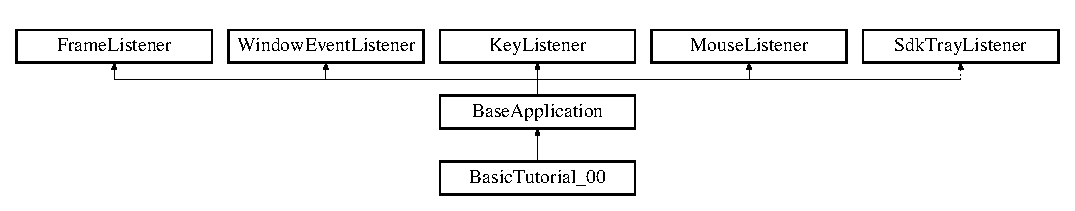
\includegraphics[height=2.382979cm]{class_base_application}
\end{center}
\end{figure}
\subsection*{Public Member Functions}
\begin{DoxyCompactItemize}
\item 
\hypertarget{class_base_application_a8a14a65a29118dd75173aa68678a05e1}{virtual void {\bfseries go} (void)}\label{class_base_application_a8a14a65a29118dd75173aa68678a05e1}

\end{DoxyCompactItemize}
\subsection*{Protected Member Functions}
\begin{DoxyCompactItemize}
\item 
\hypertarget{class_base_application_a5853d0e148cb85b0297a6885e1d33a89}{virtual bool {\bfseries setup} ()}\label{class_base_application_a5853d0e148cb85b0297a6885e1d33a89}

\item 
\hypertarget{class_base_application_a62ed46f90e9f82cc810997647a2c587e}{virtual bool {\bfseries configure} (void)}\label{class_base_application_a62ed46f90e9f82cc810997647a2c587e}

\item 
\hypertarget{class_base_application_ad5bc9655041e1849a4c13f444a3712bd}{virtual void {\bfseries choose\-Scene\-Manager} (void)}\label{class_base_application_ad5bc9655041e1849a4c13f444a3712bd}

\item 
\hypertarget{class_base_application_afa9d51527763cf9aee9cd4e1b1039d55}{virtual void {\bfseries create\-Camera} (void)}\label{class_base_application_afa9d51527763cf9aee9cd4e1b1039d55}

\item 
\hypertarget{class_base_application_aff6fd9ff1ff0978cc68f19dd65be4778}{virtual void {\bfseries create\-Frame\-Listener} (void)}\label{class_base_application_aff6fd9ff1ff0978cc68f19dd65be4778}

\item 
\hypertarget{class_base_application_aa97beeb4059b17d0ec22eae33286ec2d}{virtual void {\bfseries create\-Scene} (void)=0}\label{class_base_application_aa97beeb4059b17d0ec22eae33286ec2d}

\item 
\hypertarget{class_base_application_a365146059b25391fe400f5fdb94f011e}{virtual void {\bfseries destroy\-Scene} (void)}\label{class_base_application_a365146059b25391fe400f5fdb94f011e}

\item 
\hypertarget{class_base_application_a1f8f6730cae6ec769d8730b1af48486e}{virtual void {\bfseries create\-Viewports} (void)}\label{class_base_application_a1f8f6730cae6ec769d8730b1af48486e}

\item 
\hypertarget{class_base_application_ae27301702f1e5de64619a39b1929f1f9}{virtual void {\bfseries setup\-Resources} (void)}\label{class_base_application_ae27301702f1e5de64619a39b1929f1f9}

\item 
\hypertarget{class_base_application_a9b77972f0f747a61e1f8ceba2ad47641}{virtual void {\bfseries create\-Resource\-Listener} (void)}\label{class_base_application_a9b77972f0f747a61e1f8ceba2ad47641}

\item 
\hypertarget{class_base_application_aaeb764e637dd87601a81a80156659d88}{virtual void {\bfseries load\-Resources} (void)}\label{class_base_application_aaeb764e637dd87601a81a80156659d88}

\item 
\hypertarget{class_base_application_a03912a0f38b38fede7f08a2571e8fc56}{virtual bool {\bfseries frame\-Rendering\-Queued} (const Ogre\-::\-Frame\-Event \&evt)}\label{class_base_application_a03912a0f38b38fede7f08a2571e8fc56}

\item 
\hypertarget{class_base_application_acfa977f04e435f18018ece805c1277ec}{virtual bool {\bfseries key\-Pressed} (const O\-I\-S\-::\-Key\-Event \&arg)}\label{class_base_application_acfa977f04e435f18018ece805c1277ec}

\item 
\hypertarget{class_base_application_aba5c7c9dea7a0efc58b89310bae547e5}{virtual bool {\bfseries key\-Released} (const O\-I\-S\-::\-Key\-Event \&arg)}\label{class_base_application_aba5c7c9dea7a0efc58b89310bae547e5}

\item 
\hypertarget{class_base_application_a126e59cb246b061e51eb6ce06a2ee8f4}{virtual bool {\bfseries mouse\-Moved} (const O\-I\-S\-::\-Mouse\-Event \&arg)}\label{class_base_application_a126e59cb246b061e51eb6ce06a2ee8f4}

\item 
\hypertarget{class_base_application_a9255dfc1eabefd11c474ec45a6622504}{virtual bool {\bfseries mouse\-Pressed} (const O\-I\-S\-::\-Mouse\-Event \&arg, O\-I\-S\-::\-Mouse\-Button\-I\-D id)}\label{class_base_application_a9255dfc1eabefd11c474ec45a6622504}

\item 
\hypertarget{class_base_application_aa102c5859c14c0690c749994a446b53d}{virtual bool {\bfseries mouse\-Released} (const O\-I\-S\-::\-Mouse\-Event \&arg, O\-I\-S\-::\-Mouse\-Button\-I\-D id)}\label{class_base_application_aa102c5859c14c0690c749994a446b53d}

\item 
\hypertarget{class_base_application_afacf8a797588592ef0abbad593f10cfa}{virtual void {\bfseries window\-Resized} (Ogre\-::\-Render\-Window $\ast$rw)}\label{class_base_application_afacf8a797588592ef0abbad593f10cfa}

\item 
\hypertarget{class_base_application_ae0e37ac54a31ff6e51d58c7654ad1b90}{virtual void {\bfseries window\-Closed} (Ogre\-::\-Render\-Window $\ast$rw)}\label{class_base_application_ae0e37ac54a31ff6e51d58c7654ad1b90}

\end{DoxyCompactItemize}
\subsection*{Protected Attributes}
\begin{DoxyCompactItemize}
\item 
\hypertarget{class_base_application_add84ba707dc6c57e6283f214b1274110}{Ogre\-::\-Root $\ast$ {\bfseries m\-Root}}\label{class_base_application_add84ba707dc6c57e6283f214b1274110}

\item 
\hypertarget{class_base_application_a3829c6b12afe911e97e6b4524b33a38b}{Ogre\-::\-Camera $\ast$ {\bfseries m\-Camera}}\label{class_base_application_a3829c6b12afe911e97e6b4524b33a38b}

\item 
\hypertarget{class_base_application_a8a7684f4f9a57ed3089048ad1a913b2d}{Ogre\-::\-Scene\-Manager $\ast$ {\bfseries m\-Scene\-Mgr}}\label{class_base_application_a8a7684f4f9a57ed3089048ad1a913b2d}

\item 
\hypertarget{class_base_application_ac5d8e9c81e036897bc82f81eff8c570f}{Ogre\-::\-Render\-Window $\ast$ {\bfseries m\-Window}}\label{class_base_application_ac5d8e9c81e036897bc82f81eff8c570f}

\item 
\hypertarget{class_base_application_a765e0df01c141a16df3178ab4f17afe6}{Ogre\-::\-String {\bfseries m\-Resources\-Cfg}}\label{class_base_application_a765e0df01c141a16df3178ab4f17afe6}

\item 
\hypertarget{class_base_application_a04f2fe47fa164fd78d986dc0df70b7fb}{Ogre\-::\-String {\bfseries m\-Plugins\-Cfg}}\label{class_base_application_a04f2fe47fa164fd78d986dc0df70b7fb}

\item 
\hypertarget{class_base_application_a7faa397f4f4861ee8c361a01e90b4416}{Ogre\-Bites\-::\-Sdk\-Tray\-Manager $\ast$ {\bfseries m\-Tray\-Mgr}}\label{class_base_application_a7faa397f4f4861ee8c361a01e90b4416}

\item 
\hypertarget{class_base_application_a9ae38dea6316058549151fff66a91fcd}{Ogre\-Bites\-::\-Sdk\-Camera\-Man $\ast$ {\bfseries m\-Camera\-Man}}\label{class_base_application_a9ae38dea6316058549151fff66a91fcd}

\item 
\hypertarget{class_base_application_a6a11054ca61efdf558e0ff1b2de43a12}{Ogre\-Bites\-::\-Params\-Panel $\ast$ {\bfseries m\-Details\-Panel}}\label{class_base_application_a6a11054ca61efdf558e0ff1b2de43a12}

\item 
\hypertarget{class_base_application_ac7e861799862cb645f1d78b170aef80d}{bool {\bfseries m\-Cursor\-Was\-Visible}}\label{class_base_application_ac7e861799862cb645f1d78b170aef80d}

\item 
\hypertarget{class_base_application_a755f26d3a9915aaf830750d877e39d86}{bool {\bfseries m\-Shut\-Down}}\label{class_base_application_a755f26d3a9915aaf830750d877e39d86}

\item 
\hypertarget{class_base_application_abc9503c8462e225b5d0d55c952d9e4a9}{O\-I\-S\-::\-Input\-Manager $\ast$ {\bfseries m\-Input\-Manager}}\label{class_base_application_abc9503c8462e225b5d0d55c952d9e4a9}

\item 
\hypertarget{class_base_application_add9b97fbe64da2814d3af113bac58c43}{O\-I\-S\-::\-Mouse $\ast$ {\bfseries m\-Mouse}}\label{class_base_application_add9b97fbe64da2814d3af113bac58c43}

\item 
\hypertarget{class_base_application_a9d6e19cf50c47379fbaae55bff28079c}{O\-I\-S\-::\-Keyboard $\ast$ {\bfseries m\-Keyboard}}\label{class_base_application_a9d6e19cf50c47379fbaae55bff28079c}

\item 
\hypertarget{class_base_application_a163e5a26419ca3462d4d9aac200bd1d1}{Ogre\-Bites\-::\-Text\-Box $\ast$ {\bfseries About\-\_\-\-Text}}\label{class_base_application_a163e5a26419ca3462d4d9aac200bd1d1}

\item 
\hypertarget{class_base_application_a0ce91b17321fff8315a1c558c09316fd}{Ogre\-Bites\-::\-Label $\ast$ {\bfseries Time\-\_\-\-Show}}\label{class_base_application_a0ce91b17321fff8315a1c558c09316fd}

\item 
\hypertarget{class_base_application_a7a54628f50fbf2ffe5d983300ff9a16c}{Ogre\-Bites\-::\-Label $\ast$ {\bfseries Score\-\_\-\-Show}}\label{class_base_application_a7a54628f50fbf2ffe5d983300ff9a16c}

\item 
\hypertarget{class_base_application_a62e99e983e29fe03f77b9efff43956a1}{Ogre\-Bites\-::\-Label $\ast$ {\bfseries Time\-\_\-\-Value\-\_\-\-Show}}\label{class_base_application_a62e99e983e29fe03f77b9efff43956a1}

\item 
\hypertarget{class_base_application_a423c512b139f362e8bc1d14a72b0057d}{Ogre\-Bites\-::\-Label $\ast$ {\bfseries Score\-\_\-\-Value\-\_\-\-Show}}\label{class_base_application_a423c512b139f362e8bc1d14a72b0057d}

\item 
\hypertarget{class_base_application_acb006d144c3704c900fbaab926513be2}{Ogre\-Bites\-::\-Button $\ast$ {\bfseries Button\-\_\-\-All} \mbox{[}26\mbox{]}}\label{class_base_application_acb006d144c3704c900fbaab926513be2}

\end{DoxyCompactItemize}


The documentation for this class was generated from the following files\-:\begin{DoxyCompactItemize}
\item 
source/Base\-Application.\-h\item 
source/Base\-Application.\-cpp\end{DoxyCompactItemize}

\hypertarget{class_basic_tutorial__00}{\section{Basic\-Tutorial\-\_\-00 Class Reference}
\label{class_basic_tutorial__00}\index{Basic\-Tutorial\-\_\-00@{Basic\-Tutorial\-\_\-00}}
}


3\-D Game Programming \par
 My Name\-: Wei-\/\-Sheng Zeng , Yen-\/\-Ting Kuan \par
 My I\-D\-: 9917144 , 9917260 \par
 My Email\-: \href{mailto:cvs5689@gmail.com}{\tt cvs5689@gmail.\-com} , \href{mailto:fly19920820@yahoo.com.tw}{\tt fly19920820@yahoo.\-com.\-tw}  




{\ttfamily \#include $<$Tutorial\-Application.\-h$>$}

Inheritance diagram for Basic\-Tutorial\-\_\-00\-:\begin{figure}[H]
\begin{center}
\leavevmode
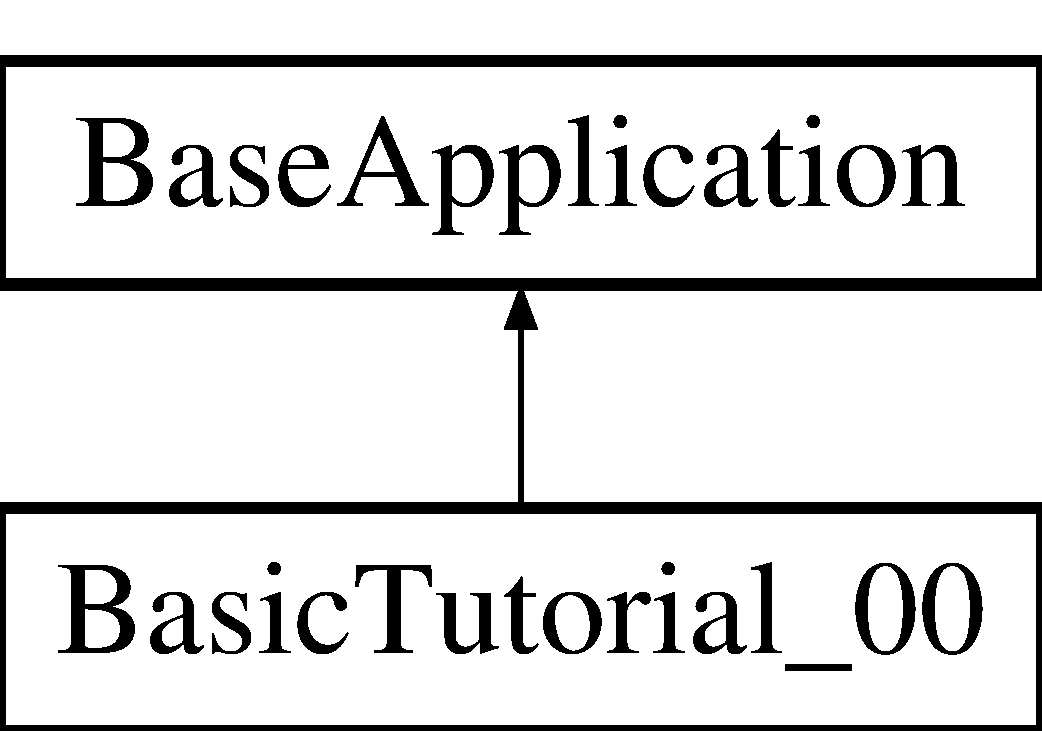
\includegraphics[height=2.382979cm]{class_basic_tutorial__00}
\end{center}
\end{figure}
\subsection*{Public Member Functions}
\begin{DoxyCompactItemize}
\item 
\hypertarget{class_basic_tutorial__00_a94e281a96584a25bf57b1c5e73737c81}{virtual bool {\bfseries frame\-Started} (const Ogre\-::\-Frame\-Event \&evt)}\label{class_basic_tutorial__00_a94e281a96584a25bf57b1c5e73737c81}

\item 
virtual void \hyperlink{class_basic_tutorial__00_adc2454d9f8226e0958ecf702f355846e}{create\-Viewports} (void)
\item 
virtual void \hyperlink{class_basic_tutorial__00_a15a3d4673724ec99077ce992f996a550}{create\-Scene} (void)
\item 
virtual void \hyperlink{class_basic_tutorial__00_a1bf709417d654dffc2ea10987412b912}{create\-Camera} (void)
\item 
virtual void \hyperlink{class_basic_tutorial__00_aba97a29d983586d2dc8e108d3bccf721}{choose\-Scene\-Manager} (void)
\item 
\hypertarget{class_basic_tutorial__00_adc1a0b32d78b1980b3ee51a1b1e1e69b}{virtual bool {\bfseries key\-Pressed} (const O\-I\-S\-::\-Key\-Event \&arg)}\label{class_basic_tutorial__00_adc1a0b32d78b1980b3ee51a1b1e1e69b}

\item 
\hypertarget{class_basic_tutorial__00_aacca7a0a2a5a0e0d007b9c6c30b4941b}{virtual bool {\bfseries key\-Released} (const O\-I\-S\-::\-Key\-Event \&arg)}\label{class_basic_tutorial__00_aacca7a0a2a5a0e0d007b9c6c30b4941b}

\item 
\hypertarget{class_basic_tutorial__00_af0e5dec72c58e157c2a63ffa5fd8c7c7}{virtual bool {\bfseries mouse\-Pressed} (const O\-I\-S\-::\-Mouse\-Event \&arg, O\-I\-S\-::\-Mouse\-Button\-I\-D id)}\label{class_basic_tutorial__00_af0e5dec72c58e157c2a63ffa5fd8c7c7}

\end{DoxyCompactItemize}
\subsection*{Additional Inherited Members}


\subsection{Detailed Description}
3\-D Game Programming \par
 My Name\-: Wei-\/\-Sheng Zeng , Yen-\/\-Ting Kuan \par
 My I\-D\-: 9917144 , 9917260 \par
 My Email\-: \href{mailto:cvs5689@gmail.com}{\tt cvs5689@gmail.\-com} , \href{mailto:fly19920820@yahoo.com.tw}{\tt fly19920820@yahoo.\-com.\-tw} 

This is an assignment of 3\-D Game Programming

All application here,include F\-S\-M,U\-I and user control. 

\subsection{Member Function Documentation}
\hypertarget{class_basic_tutorial__00_aba97a29d983586d2dc8e108d3bccf721}{\index{Basic\-Tutorial\-\_\-00@{Basic\-Tutorial\-\_\-00}!choose\-Scene\-Manager@{choose\-Scene\-Manager}}
\index{choose\-Scene\-Manager@{choose\-Scene\-Manager}!BasicTutorial_00@{Basic\-Tutorial\-\_\-00}}
\subsubsection[{choose\-Scene\-Manager}]{\setlength{\rightskip}{0pt plus 5cm}void Basic\-Tutorial\-\_\-00\-::choose\-Scene\-Manager (
\begin{DoxyParamCaption}
\item[{void}]{}
\end{DoxyParamCaption}
)\hspace{0.3cm}{\ttfamily [virtual]}}}\label{class_basic_tutorial__00_aba97a29d983586d2dc8e108d3bccf721}
Simply create two scene manager. 

Reimplemented from \hyperlink{class_base_application}{Base\-Application}.

\hypertarget{class_basic_tutorial__00_a1bf709417d654dffc2ea10987412b912}{\index{Basic\-Tutorial\-\_\-00@{Basic\-Tutorial\-\_\-00}!create\-Camera@{create\-Camera}}
\index{create\-Camera@{create\-Camera}!BasicTutorial_00@{Basic\-Tutorial\-\_\-00}}
\subsubsection[{create\-Camera}]{\setlength{\rightskip}{0pt plus 5cm}void Basic\-Tutorial\-\_\-00\-::create\-Camera (
\begin{DoxyParamCaption}
\item[{void}]{}
\end{DoxyParamCaption}
)\hspace{0.3cm}{\ttfamily [virtual]}}}\label{class_basic_tutorial__00_a1bf709417d654dffc2ea10987412b912}
Call create\-Game\-Main\-Camera and create\-Game\-Back\-Little\-Camera to setup two cameras and set camera\-\_\-00 to be main. 

Reimplemented from \hyperlink{class_base_application}{Base\-Application}.

\hypertarget{class_basic_tutorial__00_a15a3d4673724ec99077ce992f996a550}{\index{Basic\-Tutorial\-\_\-00@{Basic\-Tutorial\-\_\-00}!create\-Scene@{create\-Scene}}
\index{create\-Scene@{create\-Scene}!BasicTutorial_00@{Basic\-Tutorial\-\_\-00}}
\subsubsection[{create\-Scene}]{\setlength{\rightskip}{0pt plus 5cm}void Basic\-Tutorial\-\_\-00\-::create\-Scene (
\begin{DoxyParamCaption}
\item[{void}]{}
\end{DoxyParamCaption}
)\hspace{0.3cm}{\ttfamily [virtual]}}}\label{class_basic_tutorial__00_a15a3d4673724ec99077ce992f996a550}
Call create\-Game\-Scene and create\-Scene\-\_\-01 to create two scenes. 

Implements \hyperlink{class_base_application}{Base\-Application}.

\hypertarget{class_basic_tutorial__00_adc2454d9f8226e0958ecf702f355846e}{\index{Basic\-Tutorial\-\_\-00@{Basic\-Tutorial\-\_\-00}!create\-Viewports@{create\-Viewports}}
\index{create\-Viewports@{create\-Viewports}!BasicTutorial_00@{Basic\-Tutorial\-\_\-00}}
\subsubsection[{create\-Viewports}]{\setlength{\rightskip}{0pt plus 5cm}void Basic\-Tutorial\-\_\-00\-::create\-Viewports (
\begin{DoxyParamCaption}
\item[{void}]{}
\end{DoxyParamCaption}
)\hspace{0.3cm}{\ttfamily [virtual]}}}\label{class_basic_tutorial__00_adc2454d9f8226e0958ecf702f355846e}
Set up two viewport with create\-Game\-Main\-Viewport and create\-Game\-Back\-Little\-Viewport. 

Reimplemented from \hyperlink{class_base_application}{Base\-Application}.



The documentation for this class was generated from the following files\-:\begin{DoxyCompactItemize}
\item 
source/Tutorial\-Application.\-h\item 
source/Tutorial\-Application.\-cpp\end{DoxyCompactItemize}

\hypertarget{class_block}{\section{Block Class Reference}
\label{class_block}\index{Block@{Block}}
}


Game block for stacking,apply shape control,move,rotate here.  




{\ttfamily \#include $<$Block.\-h$>$}

\subsection*{Public Member Functions}
\begin{DoxyCompactItemize}
\item 
\hypertarget{class_block_a4bf11350657f21c4dcffe68bd624d150}{{\bfseries Block} (Scene\-Manager $\ast$a\-\_\-\-Scene\-Mgr)}\label{class_block_a4bf11350657f21c4dcffe68bd624d150}

\item 
\hypertarget{class_block_ad0a82dba858dc44e4e7dd194686cc5a8}{virtual void {\bfseries update} (const Ogre\-::\-Frame\-Event \&evt)}\label{class_block_ad0a82dba858dc44e4e7dd194686cc5a8}

\item 
\hypertarget{class_block_af2d5c039dae734db80e4b848759422d6}{virtual void {\bfseries update\-Location} ()}\label{class_block_af2d5c039dae734db80e4b848759422d6}

\item 
\hypertarget{class_block_a16c9ecdeeb71d126a00eed53083247ea}{virtual const Ogre\-::\-Vector3 \& {\bfseries get\-Position} () const }\label{class_block_a16c9ecdeeb71d126a00eed53083247ea}

\item 
\hypertarget{class_block_a352bbf7982b39bf1297747286bffe822}{virtual Ogre\-::\-Vector3 $\ast$ {\bfseries get\-All\-Position} ()}\label{class_block_a352bbf7982b39bf1297747286bffe822}

\item 
\hypertarget{class_block_ad1476f8033a35ef72e02bcaf058ae044}{virtual bool {\bfseries get\-Exist} (int num)}\label{class_block_ad1476f8033a35ef72e02bcaf058ae044}

\item 
\hypertarget{class_block_ae073b3711d637ffcb5d13edc67c6c96c}{virtual void {\bfseries set\-Visible} (bool b)}\label{class_block_ae073b3711d637ffcb5d13edc67c6c96c}

\item 
\hypertarget{class_block_ab349f41487a18a2115d47f747f722ad1}{virtual void {\bfseries set\-Position} (const Vector3 \&pos)}\label{class_block_ab349f41487a18a2115d47f747f722ad1}

\item 
\hypertarget{class_block_a739df9c84276a9a3dd1ac4e5307e6c7a}{virtual void {\bfseries translate} (const Vector3 \&v)}\label{class_block_a739df9c84276a9a3dd1ac4e5307e6c7a}

\item 
\hypertarget{class_block_ad3798370b0029774ed9eed643c708c11}{virtual void {\bfseries clear} (int num)}\label{class_block_ad3798370b0029774ed9eed643c708c11}

\item 
\hypertarget{class_block_a7d465097ab0698661f4a3110319eca43}{virtual bool {\bfseries is\-All\-Clear} ()}\label{class_block_a7d465097ab0698661f4a3110319eca43}

\item 
\hypertarget{class_block_ab0ea780ca95354a851b69db9b0e77ceb}{virtual void {\bfseries rotate} (int direction)}\label{class_block_ab0ea780ca95354a851b69db9b0e77ceb}

\item 
\hypertarget{class_block_a324d004e47f5a904b5424f36a1ddc936}{virtual void {\bfseries rotate\-Back} (int direction)}\label{class_block_a324d004e47f5a904b5424f36a1ddc936}

\item 
\hypertarget{class_block_aaf3a4b01bbd67dc79a94f79e021ab0a3}{virtual void {\bfseries set\-Particle\-Enable} (bool b)}\label{class_block_aaf3a4b01bbd67dc79a94f79e021ab0a3}

\end{DoxyCompactItemize}
\subsection*{Static Public Attributes}
\begin{DoxyCompactItemize}
\item 
\hypertarget{class_block_afe2bfaa9c9006d31f73234396c5f751b}{static const int {\bfseries R\-O\-T\-A\-T\-E\-\_\-\-N\-O\-N\-E} = 0x0000}\label{class_block_afe2bfaa9c9006d31f73234396c5f751b}

\item 
\hypertarget{class_block_aff8a81126a2c480017d0ca7c41658ab0}{static const int {\bfseries R\-O\-T\-A\-T\-E\-\_\-\-X} = 0x0001}\label{class_block_aff8a81126a2c480017d0ca7c41658ab0}

\item 
\hypertarget{class_block_a89c7d5c8e96b7826291c323eae84db1f}{static const int {\bfseries R\-O\-T\-A\-T\-E\-\_\-\-Y} = 0x0002}\label{class_block_a89c7d5c8e96b7826291c323eae84db1f}

\item 
\hypertarget{class_block_a3f6e3d496f3944aaf4fcba7311aa8147}{static const int {\bfseries R\-O\-T\-A\-T\-E\-\_\-\-Z} = 0x0004}\label{class_block_a3f6e3d496f3944aaf4fcba7311aa8147}

\item 
\hypertarget{class_block_a13803616354222a3366865a727fa5aff}{static const int {\bfseries T\-Y\-P\-E\-\_\-\-T\-E\-S\-T} = 0x0000}\label{class_block_a13803616354222a3366865a727fa5aff}

\item 
\hypertarget{class_block_aaad4eec71c1b52a039292d08b719331a}{static const int {\bfseries T\-Y\-P\-E\-\_\-\-T} = 0x0001}\label{class_block_aaad4eec71c1b52a039292d08b719331a}

\item 
\hypertarget{class_block_a0567e31a07ee22cdf0fc1711716342c8}{static const int {\bfseries T\-Y\-P\-E\-\_\-\-L} = 0x0002}\label{class_block_a0567e31a07ee22cdf0fc1711716342c8}

\item 
\hypertarget{class_block_a36af052151d2597d4c9dc59be346da22}{static const int {\bfseries T\-Y\-P\-E\-\_\-\-L\-I\-N\-E} = 0x0004}\label{class_block_a36af052151d2597d4c9dc59be346da22}

\item 
\hypertarget{class_block_aa135bf5b73c1e1eac761885182bd87d7}{static const int {\bfseries T\-Y\-P\-E\-\_\-\-S\-Q\-U\-A\-R\-E} = 0x0008}\label{class_block_aa135bf5b73c1e1eac761885182bd87d7}

\end{DoxyCompactItemize}
\subsection*{Protected Attributes}
\begin{DoxyCompactItemize}
\item 
\hypertarget{class_block_a39d1d43e2c8bb1ed61846e678ac2db50}{Scene\-Manager $\ast$ {\bfseries m\-Scene\-Mgr}}\label{class_block_a39d1d43e2c8bb1ed61846e678ac2db50}

\item 
\hypertarget{class_block_a0ccea414cd192f094f24033a01842f01}{\hyperlink{class_g_a_m_e___o_b_j}{G\-A\-M\-E\-\_\-\-O\-B\-J} $\ast$ {\bfseries m\-Main\-Block}}\label{class_block_a0ccea414cd192f094f24033a01842f01}

\item 
\hypertarget{class_block_a987d469a443bac87614d28de94afb888}{int {\bfseries m\-Type}}\label{class_block_a987d469a443bac87614d28de94afb888}

\item 
\hypertarget{class_block_a6a0e35872ead11932e19d6db2c05c70e}{Scene\-Node $\ast$ {\bfseries m\-Attached\-Block} \mbox{[}4\mbox{]}}\label{class_block_a6a0e35872ead11932e19d6db2c05c70e}

\item 
\hypertarget{class_block_af31ceac23c4ac8d54563724a4037c60a}{Vector3 {\bfseries m\-Position} \mbox{[}4\mbox{]}}\label{class_block_af31ceac23c4ac8d54563724a4037c60a}

\item 
\hypertarget{class_block_ab59a6d207ffd4a29da3c5e9e1e31cf82}{bool {\bfseries m\-Block\-Exist} \mbox{[}4\mbox{]}}\label{class_block_ab59a6d207ffd4a29da3c5e9e1e31cf82}

\item 
\hypertarget{class_block_a3fccba5f9fa086791928ef553584994e}{Scene\-Node $\ast$ {\bfseries f\-Node} \mbox{[}4\mbox{]}}\label{class_block_a3fccba5f9fa086791928ef553584994e}

\item 
\hypertarget{class_block_ad9374c927012d94bdcdad9e83a891ca3}{bool {\bfseries m\-Turned} \mbox{[}3\mbox{]}}\label{class_block_ad9374c927012d94bdcdad9e83a891ca3}

\item 
\hypertarget{class_block_a7f2f9acf4d53436a32fdfe33d106bad1}{bool {\bfseries m\-Particle\-Enabled}}\label{class_block_a7f2f9acf4d53436a32fdfe33d106bad1}

\item 
\hypertarget{class_block_a5b6bddeced665c17cd9b984f3d3ed0f6}{Real {\bfseries m\-Counter}}\label{class_block_a5b6bddeced665c17cd9b984f3d3ed0f6}

\end{DoxyCompactItemize}


\subsection{Detailed Description}
Game block for stacking,apply shape control,move,rotate here. 

The documentation for this class was generated from the following files\-:\begin{DoxyCompactItemize}
\item 
source/Block.\-h\item 
source/Block.\-cpp\end{DoxyCompactItemize}

\hypertarget{class_block_manager}{\section{Block\-Manager Class Reference}
\label{class_block_manager}\index{Block\-Manager@{Block\-Manager}}
}


\hyperlink{class_block}{Block} manager for A\-L\-L blocks,check the chess board and clear the layer that is full,also apply A\-I L\-O\-G\-I\-C Design here.  




{\ttfamily \#include $<$Block\-Manager.\-h$>$}

\subsection*{Public Member Functions}
\begin{DoxyCompactItemize}
\item 
\hypertarget{class_block_manager_a23667f9b62f96c6de25668a941fe7eec}{{\bfseries Block\-Manager} (Scene\-Manager $\ast$a\-\_\-\-Scene\-Mgr)}\label{class_block_manager_a23667f9b62f96c6de25668a941fe7eec}

\item 
\hypertarget{class_block_manager_afa3d60106faa33b29cffe60eabceb45f}{virtual void {\bfseries update} (const Ogre\-::\-Frame\-Event \&evt)}\label{class_block_manager_afa3d60106faa33b29cffe60eabceb45f}

\item 
\hypertarget{class_block_manager_af03f6328fb1c5ad2e408ae947d23c350}{virtual void {\bfseries create\-New\-Block} ()}\label{class_block_manager_af03f6328fb1c5ad2e408ae947d23c350}

\item 
\hypertarget{class_block_manager_a6c70dd950f9754a5ce4a76fb564d3beb}{virtual void {\bfseries move\-Block} (int dir)}\label{class_block_manager_a6c70dd950f9754a5ce4a76fb564d3beb}

\item 
\hypertarget{class_block_manager_a100818f16347fa6de20c7fb2c9f805a0}{virtual void {\bfseries rotate\-Block} (int dir)}\label{class_block_manager_a100818f16347fa6de20c7fb2c9f805a0}

\item 
\hypertarget{class_block_manager_a620fcc88b0a143316d84b7e77df6199e}{virtual void {\bfseries A\-I\-Plan} ()}\label{class_block_manager_a620fcc88b0a143316d84b7e77df6199e}

\item 
\hypertarget{class_block_manager_a3a90440297090de6409696c1ce1a129f}{virtual void {\bfseries A\-I\-Plan\-Logic} ()}\label{class_block_manager_a3a90440297090de6409696c1ce1a129f}

\item 
\hypertarget{class_block_manager_ab88a0f31d62055480f3798d7b2f09b6f}{virtual int {\bfseries A\-I\-Move\-Plan} ()}\label{class_block_manager_ab88a0f31d62055480f3798d7b2f09b6f}

\item 
\hypertarget{class_block_manager_aa5e7a0830d4105b4fdb7f59e58ca06b5}{virtual int {\bfseries A\-I\-Rotate\-Plan} ()}\label{class_block_manager_aa5e7a0830d4105b4fdb7f59e58ca06b5}

\item 
\hypertarget{class_block_manager_ad28546fe41da51c1e4ddfd14c8eeead8}{virtual bool {\bfseries is\-End} ()}\label{class_block_manager_ad28546fe41da51c1e4ddfd14c8eeead8}

\item 
\hypertarget{class_block_manager_ab9ed2c6d6c044417515a04beb836f7f7}{virtual int {\bfseries get\-Score} ()}\label{class_block_manager_ab9ed2c6d6c044417515a04beb836f7f7}

\item 
\hypertarget{class_block_manager_a0f52d717e79da943ff045d715cbde5fe}{virtual void {\bfseries set\-Particle\-Enabled} (bool b)}\label{class_block_manager_a0f52d717e79da943ff045d715cbde5fe}

\end{DoxyCompactItemize}
\subsection*{Static Public Attributes}
\begin{DoxyCompactItemize}
\item 
\hypertarget{class_block_manager_a768886c4d8c4e657e2212d49e204b19a}{static const int {\bfseries M\-O\-V\-E\-\_\-\-N\-O\-N\-E} = 0x0000}\label{class_block_manager_a768886c4d8c4e657e2212d49e204b19a}

\item 
\hypertarget{class_block_manager_a969530de2202f4b42f69e37060bb9a6b}{static const int {\bfseries M\-O\-V\-E\-\_\-\-U\-P} = 0x0001}\label{class_block_manager_a969530de2202f4b42f69e37060bb9a6b}

\item 
\hypertarget{class_block_manager_a59d5bae659415b234359ee927dfd86fe}{static const int {\bfseries M\-O\-V\-E\-\_\-\-D\-O\-W\-N} = 0x0002}\label{class_block_manager_a59d5bae659415b234359ee927dfd86fe}

\item 
\hypertarget{class_block_manager_afd6b587b8a0b45b915adb975c87a432e}{static const int {\bfseries M\-O\-V\-E\-\_\-\-L\-E\-F\-T} = 0x0004}\label{class_block_manager_afd6b587b8a0b45b915adb975c87a432e}

\item 
\hypertarget{class_block_manager_a86a4499f0986b5c17d6af170d4269b0c}{static const int {\bfseries M\-O\-V\-E\-\_\-\-R\-I\-G\-H\-T} = 0x0008}\label{class_block_manager_a86a4499f0986b5c17d6af170d4269b0c}

\item 
\hypertarget{class_block_manager_ac72581c347a0b65de178b4ec85105cfc}{static const int {\bfseries M\-O\-V\-E\-\_\-\-S\-P\-E\-E\-D\-U\-P} = 0x0010}\label{class_block_manager_ac72581c347a0b65de178b4ec85105cfc}

\end{DoxyCompactItemize}
\subsection*{Protected Member Functions}
\begin{DoxyCompactItemize}
\item 
\hypertarget{class_block_manager_a2b2c737776e012b5b6c2830e1d3c4da7}{void {\bfseries resolve\-Move\-Collision} (Vector3 \&pre\-Position)}\label{class_block_manager_a2b2c737776e012b5b6c2830e1d3c4da7}

\item 
\hypertarget{class_block_manager_a599c67ecfbac762fef8936e8ba47f89c}{void {\bfseries resolve\-Rotate\-Collision} (int direction)}\label{class_block_manager_a599c67ecfbac762fef8936e8ba47f89c}

\item 
\hypertarget{class_block_manager_a28c627de985af22a9efc893431954385}{bool {\bfseries resolve\-Block\-Collision} ()}\label{class_block_manager_a28c627de985af22a9efc893431954385}

\item 
\hypertarget{class_block_manager_af419044ea5a2146626b8af9beb14bba1}{bool {\bfseries resolve\-Bound\-Collision} ()}\label{class_block_manager_af419044ea5a2146626b8af9beb14bba1}

\item 
\hypertarget{class_block_manager_ae2c5327d3e1c9a6d9aaf58fb082fb9da}{void {\bfseries project\-Current\-Block} ()}\label{class_block_manager_ae2c5327d3e1c9a6d9aaf58fb082fb9da}

\item 
\hypertarget{class_block_manager_a53c2746558ef05c9eb2bfc26d5836170}{void {\bfseries record\-Location} ()}\label{class_block_manager_a53c2746558ef05c9eb2bfc26d5836170}

\item 
\hypertarget{class_block_manager_a7f8ede085348bd637eeabfb208487d0f}{void {\bfseries clear\-Block} (int layer)}\label{class_block_manager_a7f8ede085348bd637eeabfb208487d0f}

\item 
\hypertarget{class_block_manager_a6e4ef5a21263539dfd1eacf253fbaca2}{void {\bfseries setup\-Sound} (void)}\label{class_block_manager_a6e4ef5a21263539dfd1eacf253fbaca2}

\end{DoxyCompactItemize}
\subsection*{Protected Attributes}
\begin{DoxyCompactItemize}
\item 
\hypertarget{class_block_manager_a063fa719baa0dbf70ac976184be6c4a4}{int {\bfseries m\-Cur\-Blocks\-Num}}\label{class_block_manager_a063fa719baa0dbf70ac976184be6c4a4}

\item 
\hypertarget{class_block_manager_aeede5bfde3880f053bd137a03959527d}{bool {\bfseries m\-End}}\label{class_block_manager_aeede5bfde3880f053bd137a03959527d}

\item 
\hypertarget{class_block_manager_af9324df428403b998ca0f7cc261957ea}{int {\bfseries score\-\_\-plus}}\label{class_block_manager_af9324df428403b998ca0f7cc261957ea}

\item 
\hypertarget{class_block_manager_adf8b2993edb68348c6a332b32c0d0091}{bool {\bfseries m\-Block\-Used} \mbox{[}512\mbox{]}}\label{class_block_manager_adf8b2993edb68348c6a332b32c0d0091}

\item 
\hypertarget{class_block_manager_a189ed2c62d6b8a073362d50bc3eea878}{\hyperlink{class_block}{Block} $\ast$ {\bfseries m\-Block\-Arr} \mbox{[}512\mbox{]}}\label{class_block_manager_a189ed2c62d6b8a073362d50bc3eea878}

\item 
\hypertarget{class_block_manager_a74ea47f30b1e7e9a4ee79178ffd55d5c}{\hyperlink{class_block}{Block} $\ast$ {\bfseries m\-Cur\-Block}}\label{class_block_manager_a74ea47f30b1e7e9a4ee79178ffd55d5c}

\item 
\hypertarget{class_block_manager_a287f3fa8101352c798b227c476a2132d}{bool $\ast$$\ast$ {\bfseries m\-Have\-Block} \mbox{[}20\mbox{]}}\label{class_block_manager_a287f3fa8101352c798b227c476a2132d}

\item 
\hypertarget{class_block_manager_a190720e7f674d746ed2b0ae2edeb3c8a}{int {\bfseries m\-Tile\-X}}\label{class_block_manager_a190720e7f674d746ed2b0ae2edeb3c8a}

\item 
\hypertarget{class_block_manager_a4ef275284527b132d50a80a796a0efab}{int {\bfseries m\-Tile\-Y}}\label{class_block_manager_a4ef275284527b132d50a80a796a0efab}

\item 
\hypertarget{class_block_manager_a0fb42aefef329c65fbef320a964e7843}{bool {\bfseries floor\-Complete\-\_\-now}}\label{class_block_manager_a0fb42aefef329c65fbef320a964e7843}

\item 
\hypertarget{class_block_manager_a0a1950331ae423bf8cedd42364ce46de}{unsigned int {\bfseries Ex\-\_\-audio\-Id}}\label{class_block_manager_a0a1950331ae423bf8cedd42364ce46de}

\item 
\hypertarget{class_block_manager_ad93465f7f3ed619d45a36daef7b832cc}{unsigned int {\bfseries Fl\-\_\-audio\-Id}}\label{class_block_manager_ad93465f7f3ed619d45a36daef7b832cc}

\item 
\hypertarget{class_block_manager_a4bf64dd505e587f142ff1053865e1204}{bool {\bfseries initial}}\label{class_block_manager_a4bf64dd505e587f142ff1053865e1204}

\item 
\hypertarget{class_block_manager_a4a3f1df135388b827046b65215881e8e}{bool {\bfseries m\-A\-I\-Planned}}\label{class_block_manager_a4a3f1df135388b827046b65215881e8e}

\item 
\hypertarget{class_block_manager_a52e4b2b469df1fc3b0c433554a059c34}{bool {\bfseries m\-Particle\-Enabled}}\label{class_block_manager_a52e4b2b469df1fc3b0c433554a059c34}

\item 
\hypertarget{class_block_manager_a545d41a71a17b7cb07ed1e4d48e6e4d5}{int {\bfseries next\-\_\-b}}\label{class_block_manager_a545d41a71a17b7cb07ed1e4d48e6e4d5}

\item 
\hypertarget{class_block_manager_af7ff9cdb5fe822ba4ec52408130f35ef}{Real {\bfseries count\-\_\-rotate}}\label{class_block_manager_af7ff9cdb5fe822ba4ec52408130f35ef}

\item 
\hypertarget{class_block_manager_a13f850b5b9fa5240e642956c680a8e34}{Vector3 {\bfseries m\-Target\-Position}}\label{class_block_manager_a13f850b5b9fa5240e642956c680a8e34}

\item 
\hypertarget{class_block_manager_a29346e118ea50c80f02c334e7aeb6e44}{Vector3 {\bfseries m\-Shape} \mbox{[}3\mbox{]}}\label{class_block_manager_a29346e118ea50c80f02c334e7aeb6e44}

\item 
\hypertarget{class_block_manager_a0cdb92b54c9826e992ca9d5ce9b13eb9}{Scene\-Manager $\ast$ {\bfseries m\-Scene\-Mgr}}\label{class_block_manager_a0cdb92b54c9826e992ca9d5ce9b13eb9}

\item 
\hypertarget{class_block_manager_aea35f500a1e95fd0fbe7f27f08126925}{\hyperlink{class_sound_manager}{Sound\-Manager} $\ast$ {\bfseries m\-Sound\-Mgr}}\label{class_block_manager_aea35f500a1e95fd0fbe7f27f08126925}

\end{DoxyCompactItemize}


\subsection{Detailed Description}
\hyperlink{class_block}{Block} manager for A\-L\-L blocks,check the chess board and clear the layer that is full,also apply A\-I L\-O\-G\-I\-C Design here. 

The documentation for this class was generated from the following files\-:\begin{DoxyCompactItemize}
\item 
source/Block\-Manager.\-h\item 
source/Block\-Manager.\-cpp\end{DoxyCompactItemize}

\hypertarget{class_d_a_t_a___r_e_a_d_e_r}{\section{D\-A\-T\-A\-\_\-\-R\-E\-A\-D\-E\-R Class Reference}
\label{class_d_a_t_a___r_e_a_d_e_r}\index{D\-A\-T\-A\-\_\-\-R\-E\-A\-D\-E\-R@{D\-A\-T\-A\-\_\-\-R\-E\-A\-D\-E\-R}}
}


Data from outer file,read and store the value.  




{\ttfamily \#include $<$read\-\_\-data.\-h$>$}

\subsection*{Static Public Member Functions}
\begin{DoxyCompactItemize}
\item 
\hypertarget{class_d_a_t_a___r_e_a_d_e_r_a385083f4162710185c7c58425d9d9805}{static void {\bfseries read\-Data} ()}\label{class_d_a_t_a___r_e_a_d_e_r_a385083f4162710185c7c58425d9d9805}

\item 
\hypertarget{class_d_a_t_a___r_e_a_d_e_r_ae622595e5d5d4afef507b99481b4b1dd}{static int {\bfseries get\-Tile\-X} ()}\label{class_d_a_t_a___r_e_a_d_e_r_ae622595e5d5d4afef507b99481b4b1dd}

\item 
\hypertarget{class_d_a_t_a___r_e_a_d_e_r_aa260b6f0016c268d63a57bb5d15c41bf}{static int {\bfseries get\-Tile\-Y} ()}\label{class_d_a_t_a___r_e_a_d_e_r_aa260b6f0016c268d63a57bb5d15c41bf}

\item 
\hypertarget{class_d_a_t_a___r_e_a_d_e_r_a2f0171b1165484f1aeade8c7f87f16ff}{static std\-::string {\bfseries get\-Back\-Music} ()}\label{class_d_a_t_a___r_e_a_d_e_r_a2f0171b1165484f1aeade8c7f87f16ff}

\end{DoxyCompactItemize}
\subsection*{Static Protected Attributes}
\begin{DoxyCompactItemize}
\item 
\hypertarget{class_d_a_t_a___r_e_a_d_e_r_ad29377b4f107485f212adf6a91fc1309}{static int {\bfseries m\-Tile\-X} = 5}\label{class_d_a_t_a___r_e_a_d_e_r_ad29377b4f107485f212adf6a91fc1309}

\item 
\hypertarget{class_d_a_t_a___r_e_a_d_e_r_a3e3642a217263d3c4ae86abd489b8a06}{static int {\bfseries m\-Tile\-Y} = 5}\label{class_d_a_t_a___r_e_a_d_e_r_a3e3642a217263d3c4ae86abd489b8a06}

\item 
\hypertarget{class_d_a_t_a___r_e_a_d_e_r_ae4db6169d844fc33d6815119a4ba79c8}{static std\-::string {\bfseries mback\-Music} = \char`\"{}\char`\"{}}\label{class_d_a_t_a___r_e_a_d_e_r_ae4db6169d844fc33d6815119a4ba79c8}

\end{DoxyCompactItemize}


\subsection{Detailed Description}
Data from outer file,read and store the value. 

The documentation for this class was generated from the following files\-:\begin{DoxyCompactItemize}
\item 
source/read\-\_\-data.\-h\item 
source/read\-\_\-data.\-cpp\end{DoxyCompactItemize}

\hypertarget{class_g_a_m_e___o_b_j}{\section{G\-A\-M\-E\-\_\-\-O\-B\-J Class Reference}
\label{class_g_a_m_e___o_b_j}\index{G\-A\-M\-E\-\_\-\-O\-B\-J@{G\-A\-M\-E\-\_\-\-O\-B\-J}}
}


Core of \hyperlink{class_block}{Block} used for control.  




{\ttfamily \#include $<$game\-\_\-obj.\-h$>$}

\subsection*{Public Member Functions}
\begin{DoxyCompactItemize}
\item 
\hypertarget{class_g_a_m_e___o_b_j_a6f0bcfa20d9187abfe3960f4df04cec4}{{\bfseries G\-A\-M\-E\-\_\-\-O\-B\-J} (Scene\-Manager $\ast$a\-\_\-\-Scene\-Mgr)}\label{class_g_a_m_e___o_b_j_a6f0bcfa20d9187abfe3960f4df04cec4}

\item 
\hypertarget{class_g_a_m_e___o_b_j_a013242ff24c23b943759280591ece4d6}{virtual void {\bfseries create\-Game\-Obj} (const String \&a\-\_\-\-Name, const String \&a\-\_\-\-Mesh\-Name)}\label{class_g_a_m_e___o_b_j_a013242ff24c23b943759280591ece4d6}

\item 
\hypertarget{class_g_a_m_e___o_b_j_ad6fcccdeb18391806452db356b479bee}{virtual void {\bfseries set\-Target} (\hyperlink{class_g_a_m_e___o_b_j}{G\-A\-M\-E\-\_\-\-O\-B\-J} $\ast$a\-\_\-\-Target)}\label{class_g_a_m_e___o_b_j_ad6fcccdeb18391806452db356b479bee}

\item 
\hypertarget{class_g_a_m_e___o_b_j_ac87e275bf68c911e4d64785d2a3836e5}{Scene\-Node $\ast$ {\bfseries get\-Scene\-Node} ()}\label{class_g_a_m_e___o_b_j_ac87e275bf68c911e4d64785d2a3836e5}

\item 
\hypertarget{class_g_a_m_e___o_b_j_a5a124501753fee239e83210cb255cdc2}{const Vector3 \& {\bfseries get\-Position} () const }\label{class_g_a_m_e___o_b_j_a5a124501753fee239e83210cb255cdc2}

\item 
\hypertarget{class_g_a_m_e___o_b_j_ab0c335efcbb8f80bb897a92441168f5e}{const Vector3 \& {\bfseries get\-Init\-Position} () const }\label{class_g_a_m_e___o_b_j_ab0c335efcbb8f80bb897a92441168f5e}

\item 
\hypertarget{class_g_a_m_e___o_b_j_a2e6d96dcfc917dcfc7fd3bf07ab3e27d}{void {\bfseries translate} (const Vector3 \&v)}\label{class_g_a_m_e___o_b_j_a2e6d96dcfc917dcfc7fd3bf07ab3e27d}

\item 
\hypertarget{class_g_a_m_e___o_b_j_aa375564b6140c1f95b76a7748dac9a74}{void {\bfseries scale} (Real sx, Real sy, Real sz)}\label{class_g_a_m_e___o_b_j_aa375564b6140c1f95b76a7748dac9a74}

\item 
\hypertarget{class_g_a_m_e___o_b_j_a8b291edd1e484532e6930feae8154257}{virtual void {\bfseries update} (const Ogre\-::\-Frame\-Event \&evt)}\label{class_g_a_m_e___o_b_j_a8b291edd1e484532e6930feae8154257}

\item 
\hypertarget{class_g_a_m_e___o_b_j_a63f209ed6267da656c9a9cb268ad1a4e}{bool {\bfseries is\-Alive} () const }\label{class_g_a_m_e___o_b_j_a63f209ed6267da656c9a9cb268ad1a4e}

\item 
\hypertarget{class_g_a_m_e___o_b_j_a98182473ba8305da60c3f8a0fe8f2bdf}{void {\bfseries make\-Alive} (bool flg=true)}\label{class_g_a_m_e___o_b_j_a98182473ba8305da60c3f8a0fe8f2bdf}

\item 
\hypertarget{class_g_a_m_e___o_b_j_a0414bbb98f31b40e73454fd01e9eeae2}{void {\bfseries set\-Life} (Real c\-Life, Real c\-Max\-Life=-\/1)}\label{class_g_a_m_e___o_b_j_a0414bbb98f31b40e73454fd01e9eeae2}

\item 
\hypertarget{class_g_a_m_e___o_b_j_a6ec6b1f338b4d6c7117b3e8f9f05029e}{void {\bfseries set\-Position} (const Vector3 \&pos)}\label{class_g_a_m_e___o_b_j_a6ec6b1f338b4d6c7117b3e8f9f05029e}

\item 
\hypertarget{class_g_a_m_e___o_b_j_ac106b5c662073f8e96cc66d96ee20285}{void {\bfseries set\-Init\-Position} (const Vector3 \&pos)}\label{class_g_a_m_e___o_b_j_ac106b5c662073f8e96cc66d96ee20285}

\item 
\hypertarget{class_g_a_m_e___o_b_j_af1e5d350761d9769632fd2d6462f6d1b}{void {\bfseries set\-Velocity} (const Vector3 \&v)}\label{class_g_a_m_e___o_b_j_af1e5d350761d9769632fd2d6462f6d1b}

\item 
\hypertarget{class_g_a_m_e___o_b_j_aaf30a973f5361ff2ba4a0d99b3966aed}{void {\bfseries set\-Speed\-Factor} (Real f)}\label{class_g_a_m_e___o_b_j_aaf30a973f5361ff2ba4a0d99b3966aed}

\item 
\hypertarget{class_g_a_m_e___o_b_j_a7db01e4e1a9baff3efdc1d77cff5dd78}{void {\bfseries set\-Visibility\-Flags} (unsigned int m)}\label{class_g_a_m_e___o_b_j_a7db01e4e1a9baff3efdc1d77cff5dd78}

\item 
\hypertarget{class_g_a_m_e___o_b_j_aec2125e20b74494704dbb32047e25bfb}{void {\bfseries set\-Visible} (bool flg)}\label{class_g_a_m_e___o_b_j_aec2125e20b74494704dbb32047e25bfb}

\end{DoxyCompactItemize}
\subsection*{Public Attributes}
\begin{DoxyCompactItemize}
\item 
\hypertarget{class_g_a_m_e___o_b_j_acd66a90f92e8882636e79e3f973124b4}{Entity $\ast$ {\bfseries m\-Entity}}\label{class_g_a_m_e___o_b_j_acd66a90f92e8882636e79e3f973124b4}

\end{DoxyCompactItemize}
\subsection*{Protected Attributes}
\begin{DoxyCompactItemize}
\item 
\hypertarget{class_g_a_m_e___o_b_j_a6fad18ad7aa1d24d6c1f873f3eaa0e30}{Scene\-Manager $\ast$ {\bfseries m\-Scene\-Mgr}}\label{class_g_a_m_e___o_b_j_a6fad18ad7aa1d24d6c1f873f3eaa0e30}

\item 
\hypertarget{class_g_a_m_e___o_b_j_a691482570994636e9fdf9bd9c7649f0b}{Scene\-Node $\ast$ {\bfseries m\-Scene\-Node}}\label{class_g_a_m_e___o_b_j_a691482570994636e9fdf9bd9c7649f0b}

\item 
\hypertarget{class_g_a_m_e___o_b_j_a3bf7eb6a27aa1490a05f5f00db5eed4b}{Real {\bfseries m\-Radius}}\label{class_g_a_m_e___o_b_j_a3bf7eb6a27aa1490a05f5f00db5eed4b}

\item 
\hypertarget{class_g_a_m_e___o_b_j_a7a2a13b6be28ffb215f49c915fa537e2}{Real {\bfseries m\-Mass}}\label{class_g_a_m_e___o_b_j_a7a2a13b6be28ffb215f49c915fa537e2}

\item 
\hypertarget{class_g_a_m_e___o_b_j_a7fd6c2fc09d900435bc20d590ab1170d}{Vector3 {\bfseries m\-Velocity}}\label{class_g_a_m_e___o_b_j_a7fd6c2fc09d900435bc20d590ab1170d}

\item 
\hypertarget{class_g_a_m_e___o_b_j_afe56a868207deaad652a56fb63786ebe}{Real {\bfseries m\-Speed\-Factor}}\label{class_g_a_m_e___o_b_j_afe56a868207deaad652a56fb63786ebe}

\item 
\hypertarget{class_g_a_m_e___o_b_j_a7547e49b1d6162044e1c8a5670bdf52e}{Quaternion {\bfseries m\-Quaternion}}\label{class_g_a_m_e___o_b_j_a7547e49b1d6162044e1c8a5670bdf52e}

\item 
\hypertarget{class_g_a_m_e___o_b_j_a7604343f0f80c8028ada3f21007e77f0}{Vector3 {\bfseries m\-Init\-Direction}}\label{class_g_a_m_e___o_b_j_a7604343f0f80c8028ada3f21007e77f0}

\item 
\hypertarget{class_g_a_m_e___o_b_j_a7a965e4b5f428fbf79544c72f1dafed7}{Vector3 {\bfseries m\-Init\-Position}}\label{class_g_a_m_e___o_b_j_a7a965e4b5f428fbf79544c72f1dafed7}

\item 
\hypertarget{class_g_a_m_e___o_b_j_a81573c1b47da8b13f5cb3f019996133a}{unsigned int {\bfseries m\-Action\-Mode}}\label{class_g_a_m_e___o_b_j_a81573c1b47da8b13f5cb3f019996133a}

\item 
\hypertarget{class_g_a_m_e___o_b_j_a9e7399dfeebe550871fc8aa9ff08d15b}{unsigned int {\bfseries m\-Fire\-Action\-Mode}}\label{class_g_a_m_e___o_b_j_a9e7399dfeebe550871fc8aa9ff08d15b}

\item 
\hypertarget{class_g_a_m_e___o_b_j_a06cd2ee5af1a884e096be40ca5e77e41}{Real {\bfseries m\-Life\-Time}}\label{class_g_a_m_e___o_b_j_a06cd2ee5af1a884e096be40ca5e77e41}

\item 
\hypertarget{class_g_a_m_e___o_b_j_a7e0a593d6273fdf6bb50b83e81ca5208}{Real {\bfseries m\-Max\-Life\-Time}}\label{class_g_a_m_e___o_b_j_a7e0a593d6273fdf6bb50b83e81ca5208}

\item 
\hypertarget{class_g_a_m_e___o_b_j_a42022f7440233c4f697e476e5fdce744}{bool {\bfseries m\-Is\-Alive}}\label{class_g_a_m_e___o_b_j_a42022f7440233c4f697e476e5fdce744}

\item 
\hypertarget{class_g_a_m_e___o_b_j_a70f8e8f74573160abc8ffd6373d2e193}{Real {\bfseries m\-Rand\-Speed}}\label{class_g_a_m_e___o_b_j_a70f8e8f74573160abc8ffd6373d2e193}

\item 
\hypertarget{class_g_a_m_e___o_b_j_ab798cf1f5d4c2411163facccb57b33e6}{Real {\bfseries m\-Time}}\label{class_g_a_m_e___o_b_j_ab798cf1f5d4c2411163facccb57b33e6}

\item 
\hypertarget{class_g_a_m_e___o_b_j_afe5eb59c2eb8bda9d96fe79f3eb7893c}{Real {\bfseries m\-Amplitude}}\label{class_g_a_m_e___o_b_j_afe5eb59c2eb8bda9d96fe79f3eb7893c}

\item 
\hypertarget{class_g_a_m_e___o_b_j_a5a0e21e5c5f78788a31506cf7ff813a3}{\hyperlink{class_g_a_m_e___o_b_j}{G\-A\-M\-E\-\_\-\-O\-B\-J} $\ast$ {\bfseries m\-Target}}\label{class_g_a_m_e___o_b_j_a5a0e21e5c5f78788a31506cf7ff813a3}

\item 
\hypertarget{class_g_a_m_e___o_b_j_afb32c5a54e7c1c481b9cbbd2c0c3f2ad}{Animation\-State $\ast$ {\bfseries m\-Animation\-State}}\label{class_g_a_m_e___o_b_j_afb32c5a54e7c1c481b9cbbd2c0c3f2ad}

\end{DoxyCompactItemize}


\subsection{Detailed Description}
Core of \hyperlink{class_block}{Block} used for control. 

The documentation for this class was generated from the following files\-:\begin{DoxyCompactItemize}
\item 
source/game\-\_\-obj.\-h\item 
source/game\-\_\-obj.\-cpp\end{DoxyCompactItemize}

\hypertarget{class_sound_manager}{\section{Sound\-Manager Class Reference}
\label{class_sound_manager}\index{Sound\-Manager@{Sound\-Manager}}
}
\subsection*{Public Member Functions}
\begin{DoxyCompactItemize}
\item 
\hypertarget{class_sound_manager_af2c2429cfe27a2a12cc2edbd9dc21d5f}{void {\bfseries self\-Destruct} (void)}\label{class_sound_manager_af2c2429cfe27a2a12cc2edbd9dc21d5f}

\item 
\hypertarget{class_sound_manager_ae47c851f33f89439e14bd2af4ff509b5}{bool {\bfseries init} (void)}\label{class_sound_manager_ae47c851f33f89439e14bd2af4ff509b5}

\item 
\hypertarget{class_sound_manager_a8e4feb6d4ecc6f14b6c7a2980e3ffbd4}{bool {\bfseries get\-Is\-Sound\-On} (void)}\label{class_sound_manager_a8e4feb6d4ecc6f14b6c7a2980e3ffbd4}

\item 
\hypertarget{class_sound_manager_aae8a2bf6adbc0a0db77bce8cfcea84a1}{void {\bfseries set\-Audio\-Path} (char $\ast$path)}\label{class_sound_manager_aae8a2bf6adbc0a0db77bce8cfcea84a1}

\item 
\hypertarget{class_sound_manager_a9168db2a3f35a33309528ea2d822a7f9}{bool {\bfseries check\-A\-L\-Error} (void)}\label{class_sound_manager_a9168db2a3f35a33309528ea2d822a7f9}

\item 
\hypertarget{class_sound_manager_a064ebf9f1c4d8c70cf8a4e01ebe17bbf}{bool {\bfseries check\-A\-L\-Error} (std\-::string p\-Msg)}\label{class_sound_manager_a064ebf9f1c4d8c70cf8a4e01ebe17bbf}

\item 
std\-::string \hyperlink{class_sound_manager_a1d4149f97293a06e51e701da4822c47e}{list\-Available\-Devices} (void)
\item 
\hypertarget{class_sound_manager_a6c83bcf9a3441a6ee2230b721e28e238}{void {\bfseries test\-Sound} (const char $\ast$wav\-File)}\label{class_sound_manager_a6c83bcf9a3441a6ee2230b721e28e238}

\item 
\hypertarget{class_sound_manager_ac3ac90d23ae5d52f74c6d625830cad5a}{bool {\bfseries load\-Audio} (std\-::string filename, unsigned int $\ast$audio\-Id, bool loop)}\label{class_sound_manager_ac3ac90d23ae5d52f74c6d625830cad5a}

\item 
\hypertarget{class_sound_manager_ae8638223cb0e8565b4f485ad56bccd03}{bool {\bfseries release\-Audio} (unsigned int audio\-I\-D)}\label{class_sound_manager_ae8638223cb0e8565b4f485ad56bccd03}

\item 
\hypertarget{class_sound_manager_a8a128ed586a43f323e41d7adaf030f33}{bool {\bfseries aquire\-Audio\-Source} (char $\ast$file, unsigned int $\ast$audio\-Id)}\label{class_sound_manager_a8a128ed586a43f323e41d7adaf030f33}

\item 
\hypertarget{class_sound_manager_a1e50bd120f94144365392bf5a163dab6}{bool {\bfseries play\-Audio} (unsigned int audio\-Id, bool force\-Restart)}\label{class_sound_manager_a1e50bd120f94144365392bf5a163dab6}

\item 
\hypertarget{class_sound_manager_a687c3db1d9d1130f9590d70d9a9f5fb5}{bool {\bfseries stop\-Audio} (unsigned int audio\-I\-D)}\label{class_sound_manager_a687c3db1d9d1130f9590d70d9a9f5fb5}

\item 
\hypertarget{class_sound_manager_ac343b4492343f4c75be9d8539a790394}{bool {\bfseries stop\-All\-Audio} (void)}\label{class_sound_manager_ac343b4492343f4c75be9d8539a790394}

\item 
\hypertarget{class_sound_manager_a01f631fd582786354869b7ffcc58f720}{bool {\bfseries pause\-Audio} (unsigned int audio\-I\-D)}\label{class_sound_manager_a01f631fd582786354869b7ffcc58f720}

\item 
\hypertarget{class_sound_manager_a2e52fa130bf73597bfe3341551812bdc}{bool {\bfseries pause\-All\-Audio} (void)}\label{class_sound_manager_a2e52fa130bf73597bfe3341551812bdc}

\item 
\hypertarget{class_sound_manager_a9f52b92c77c708a09a90d3565d9411c3}{bool {\bfseries resume\-Audio} (unsigned int audio\-I\-D)}\label{class_sound_manager_a9f52b92c77c708a09a90d3565d9411c3}

\item 
\hypertarget{class_sound_manager_a44565f0638e3a28e366aaa65ae3f1d56}{bool {\bfseries resume\-All\-Audio} (void)}\label{class_sound_manager_a44565f0638e3a28e366aaa65ae3f1d56}

\item 
\hypertarget{class_sound_manager_a4c7511ce64e05c840f94be41ccc32601}{bool {\bfseries set\-Sound\-Position} (unsigned int audio\-I\-D, Vector3 position)}\label{class_sound_manager_a4c7511ce64e05c840f94be41ccc32601}

\item 
\hypertarget{class_sound_manager_a21b37c2f591620e09cce87773fb21d32}{bool {\bfseries set\-Sound\-Position} (unsigned int audio\-I\-D, Vector3 position, Vector3 velocity, Vector3 direction)}\label{class_sound_manager_a21b37c2f591620e09cce87773fb21d32}

\item 
\hypertarget{class_sound_manager_a5072e2bd61b53cfa7a138120a5ea7404}{bool {\bfseries set\-Sound} (unsigned int audio\-I\-D, Vector3 position, Vector3 velocity, Vector3 direction, float max\-Distance, bool play\-Now, bool force\-Restart, float min\-Gain)}\label{class_sound_manager_a5072e2bd61b53cfa7a138120a5ea7404}

\item 
\hypertarget{class_sound_manager_a0ad7051e7bb37943ebdeda2d55c43798}{bool {\bfseries set\-Listener\-Position} (Vector3 position, Vector3 velocity, Quaternion orientation)}\label{class_sound_manager_a0ad7051e7bb37943ebdeda2d55c43798}

\item 
\hypertarget{class_sound_manager_a6dd06b089f7540c57d1d3a46fa843f90}{bool {\bfseries is\-Ogg\-Extension\-Present} (void)}\label{class_sound_manager_a6dd06b089f7540c57d1d3a46fa843f90}

\item 
bool \hyperlink{class_sound_manager_ae84fd5609aea7d7eef8fb92442ea92f1}{load\-Default\-Sounds} (std\-::string filename)
\item 
\hypertarget{class_sound_manager_a122cf811c2e3437585f440fb9d50da71}{void {\bfseries trim\-Trailing\-Space} (char $\ast$s)}\label{class_sound_manager_a122cf811c2e3437585f440fb9d50da71}

\end{DoxyCompactItemize}
\subsection*{Static Public Member Functions}
\begin{DoxyCompactItemize}
\item 
\hypertarget{class_sound_manager_a6ca92970a4f8c3321ddbbcc8b574654d}{static \hyperlink{class_sound_manager}{Sound\-Manager} $\ast$ {\bfseries create\-Manager} (void)}\label{class_sound_manager_a6ca92970a4f8c3321ddbbcc8b574654d}

\item 
\hypertarget{class_sound_manager_a1ff554c0e8add31b81dbc2fb6c77ed17}{static \hyperlink{class_sound_manager}{Sound\-Manager} $\ast$ {\bfseries get\-Singleton\-Ptr} (void)}\label{class_sound_manager_a1ff554c0e8add31b81dbc2fb6c77ed17}

\end{DoxyCompactItemize}
\subsection*{Static Public Attributes}
\begin{DoxyCompactItemize}
\item 
static \hyperlink{class_sound_manager}{Sound\-Manager} $\ast$ \hyperlink{class_sound_manager_ac5f215ad5ed295dcd15ebed201857d1e}{m\-Sound\-Manager} = N\-U\-L\-L
\end{DoxyCompactItemize}


\subsection{Member Function Documentation}
\hypertarget{class_sound_manager_a1d4149f97293a06e51e701da4822c47e}{\index{Sound\-Manager@{Sound\-Manager}!list\-Available\-Devices@{list\-Available\-Devices}}
\index{list\-Available\-Devices@{list\-Available\-Devices}!SoundManager@{Sound\-Manager}}
\subsubsection[{list\-Available\-Devices}]{\setlength{\rightskip}{0pt plus 5cm}std\-::string Sound\-Manager\-::list\-Available\-Devices (
\begin{DoxyParamCaption}
\item[{void}]{}
\end{DoxyParamCaption}
)}}\label{class_sound_manager_a1d4149f97293a06e51e701da4822c47e}
See \href{http://www.openal.org/windows_enumeration.html}{\tt http\-://www.\-openal.\-org/windows\-\_\-enumeration.\-html} for installing other devices. You should at least have \char`\"{}\-Generic Hardware\char`\"{}. \hypertarget{class_sound_manager_ae84fd5609aea7d7eef8fb92442ea92f1}{\index{Sound\-Manager@{Sound\-Manager}!load\-Default\-Sounds@{load\-Default\-Sounds}}
\index{load\-Default\-Sounds@{load\-Default\-Sounds}!SoundManager@{Sound\-Manager}}
\subsubsection[{load\-Default\-Sounds}]{\setlength{\rightskip}{0pt plus 5cm}bool Sound\-Manager\-::load\-Default\-Sounds (
\begin{DoxyParamCaption}
\item[{std\-::string}]{filename}
\end{DoxyParamCaption}
)}}\label{class_sound_manager_ae84fd5609aea7d7eef8fb92442ea92f1}
Preload audio files into the system. Not obligatory, the files can also be loaded on the fly. 

\subsection{Member Data Documentation}
\hypertarget{class_sound_manager_ac5f215ad5ed295dcd15ebed201857d1e}{\index{Sound\-Manager@{Sound\-Manager}!m\-Sound\-Manager@{m\-Sound\-Manager}}
\index{m\-Sound\-Manager@{m\-Sound\-Manager}!SoundManager@{Sound\-Manager}}
\subsubsection[{m\-Sound\-Manager}]{\setlength{\rightskip}{0pt plus 5cm}{\bf Sound\-Manager} $\ast$ Sound\-Manager\-::m\-Sound\-Manager = N\-U\-L\-L\hspace{0.3cm}{\ttfamily [static]}}}\label{class_sound_manager_ac5f215ad5ed295dcd15ebed201857d1e}
Sound\-Manager.\-cpp

Original Code \-: Van Stokes, Jr. (\href{http://www.EvilMasterMindsInc.com}{\tt http\-://www.\-Evil\-Master\-Minds\-Inc.\-com}) -\/ Aug 05 Modified Code \-: Steven Gay -\/ \href{mailto:mec3@bluewin.ch}{\tt mec3@bluewin.\-ch} -\/ Septembre 2005 

The documentation for this class was generated from the following files\-:\begin{DoxyCompactItemize}
\item 
source/Sound\-Manager.\-h\item 
source/Sound\-Manager.\-cpp\end{DoxyCompactItemize}

\addcontentsline{toc}{part}{Index}
\printindex
\end{document}
